
%We test this hypothesis by comparing baseline languages to \emph{fixed-order} versions of the real languages.
%This enables us to tease apart the impact of the languages' word order rules from the impact of word order freedom.


Above, we found that the majority of languages exhibit more favorable memory--surprisal trade-offs than counterfactual baselines based on random word order grammars. We also found that the strength of the difference between the real and baseline languages varies from language to language. Furthermore, we found that the magnitude of the difference is larger for languages with a higher degree of word order flexibility.


% Two issues: Confound because of restrictive formalism. 
% Association of efficiency and word order: By including information structure, we make the baselines worse
% Different orders based on info structure -> higher entropy when you don't have info structure

% Two controls:
% 1. Fixed-order baseline
% 2. Include info structure in the baseline, so that the baseline gets higher-entropy

Here, we take up the idea that 

We now address points raised above by 



\begin{enumerate}
\item First, to ensure that results are not due to the representational restrictions of the word order grammar formalism, we compare the real languages to the result of ordering the corpora according to grammars that approximates the observed orders to the extent possible in the grammar formalism.
These grammars have exactly the same representational constraints as the baseline grammars.
Importantly, they differ from real languages in having entirely deterministic order.
We expect these grammars to have better memory-surprisal tradeoffs than comparable random baseline grammars across all languages.

\item 
Languages with flexible word order often show a strong influence of information structure on word order.
Only relatively few datasets have annotations for information structure, and even fewer datasets have both syntactic and information structure annotation.
We draw on the Prague Dependency Treebank of Czech, which has both types of annotation.
Czech is a language with relatively high degree of word order freedom.

Simulation taking information structure into account (for one language).
Due to the difficulty of annotating information structure, few such corpora are available.
We use the Prague Dependency Treebank, which has information structure annotation.
\end{enumerate}




\subsection{Setup}

Everything is identical to Experiment 1, except that we replaced the real orderings with orderings generated from grammars fitted to the word orders found in the real language.

\paragraph{Fitting Ordering Grammars to Actual Orders}
We create ordering grammars that are fit to the actual orderings of each language.
These grammars faithfully represent the ordering rules if the actual language, to the extent that is possible in the formalism of ordering grammars.

We construct these grammars by constructing \emph{probabilistic ordering grammars}, and setting the parameters to maximize the \emph{likelihood} of the actually observed orderings.
The method is fully taken from \cite{hahn-universals-2020}.
%We parameterized probabilistic ordering grammars as follows.
%For each relation type $\tau$, we introduce a \emph{direction parameter} $a_\tau \in [0,1]$ and a \emph{distance parameter} $b_\tau \in \mathbb{R}$.
%Each dependent is ordered on the left of its head with probability $a_\tau$ and to the right with probability $1-a_\tau$. 
%Then for each set of co-dependents $\{s_1, \dots , s_n\}$ placed on one side of a head, their order outward from the head is determined by iteratively sampling from the distribution $\operatorname{softmax}(b_{\tau_1}, \dots, b_{\tau_n})$ (\cite{goodfellow2016deep}, p. 184) without replacement. 
%Given a dependency tree, a probabilistic ordering grammar assigns a probability distribution over the possible projective linearizations of that tree.
%We use gradient descent to find parameters $a_\tau, b_\tau$ so as to maximize the overall likelihood of the orders in the actual corpus.
%We convert probabilistic ordering grammars into ordinary ordering grammars by the following method.
%Let $A_-$ be those relations $\tau$ where $a_\tau > 0.5$, similarly for $A_+$ those here $a_\tau \geq 0.5$.
%Then we order all relations in $A_-$ by $b_\tau$ in \emph{decreasing} order, and those in $A_+$ by $b_\tau$ in \emph{increasing} order.
%Then ordering a tree following the converted version is equivalent to greedily choosing the highest-probability linearization for the dependents of each head in a tree.
%We choose this method since maximum-likelihood grammars can be constructed with simple gradient descent.
%Another option would be to use some kind of discrete optimization method to approximate the original orders without a probabilistic method.
%However, discrete optimization is computationally challenging.


\paragraph{Taking Information Structure into Account}

Part of the the Prague Dependency Treebank has annotation for topic-focus articulation \cite{mikulova2006annotation}.
Constituents are annotated for contrastiveness and for contextual boundedness, i.e., givenness.
Three labels are used:
``c'' for contrastive and contextually bound, ``f'' for contextually non-bound, ``t'' for non-contrastive contextually bound.
These labels are diagnosed based on constituent order and intonation.
Some constituents remain unmarked, the vast majority of these are function words such as adpositions, conjunctions, and auxiliaries; we introduce a label ``NA'' for these.

We extend the word order grammar formalism by defining separate weights for each combination of the 37 syntactic relations and these four information structure labels.

We obtained 38,727 training sentences and 5,228 dev sentences.


\subsection{Results}

\paragraph{Fitted Grammars}

We show estimated tradeoffs in Figure (XX).

In X languages, the fitted grammars provide better tradeoffs than at least 50\% of the random grammars.

The AUC is lower than more than 50\% of random baseline grammars in all 54 languages ($p < 0.01$, using two-sided Binomial test and Hochberg's step-up procedure).


\begin{figure}
	\begin{center}
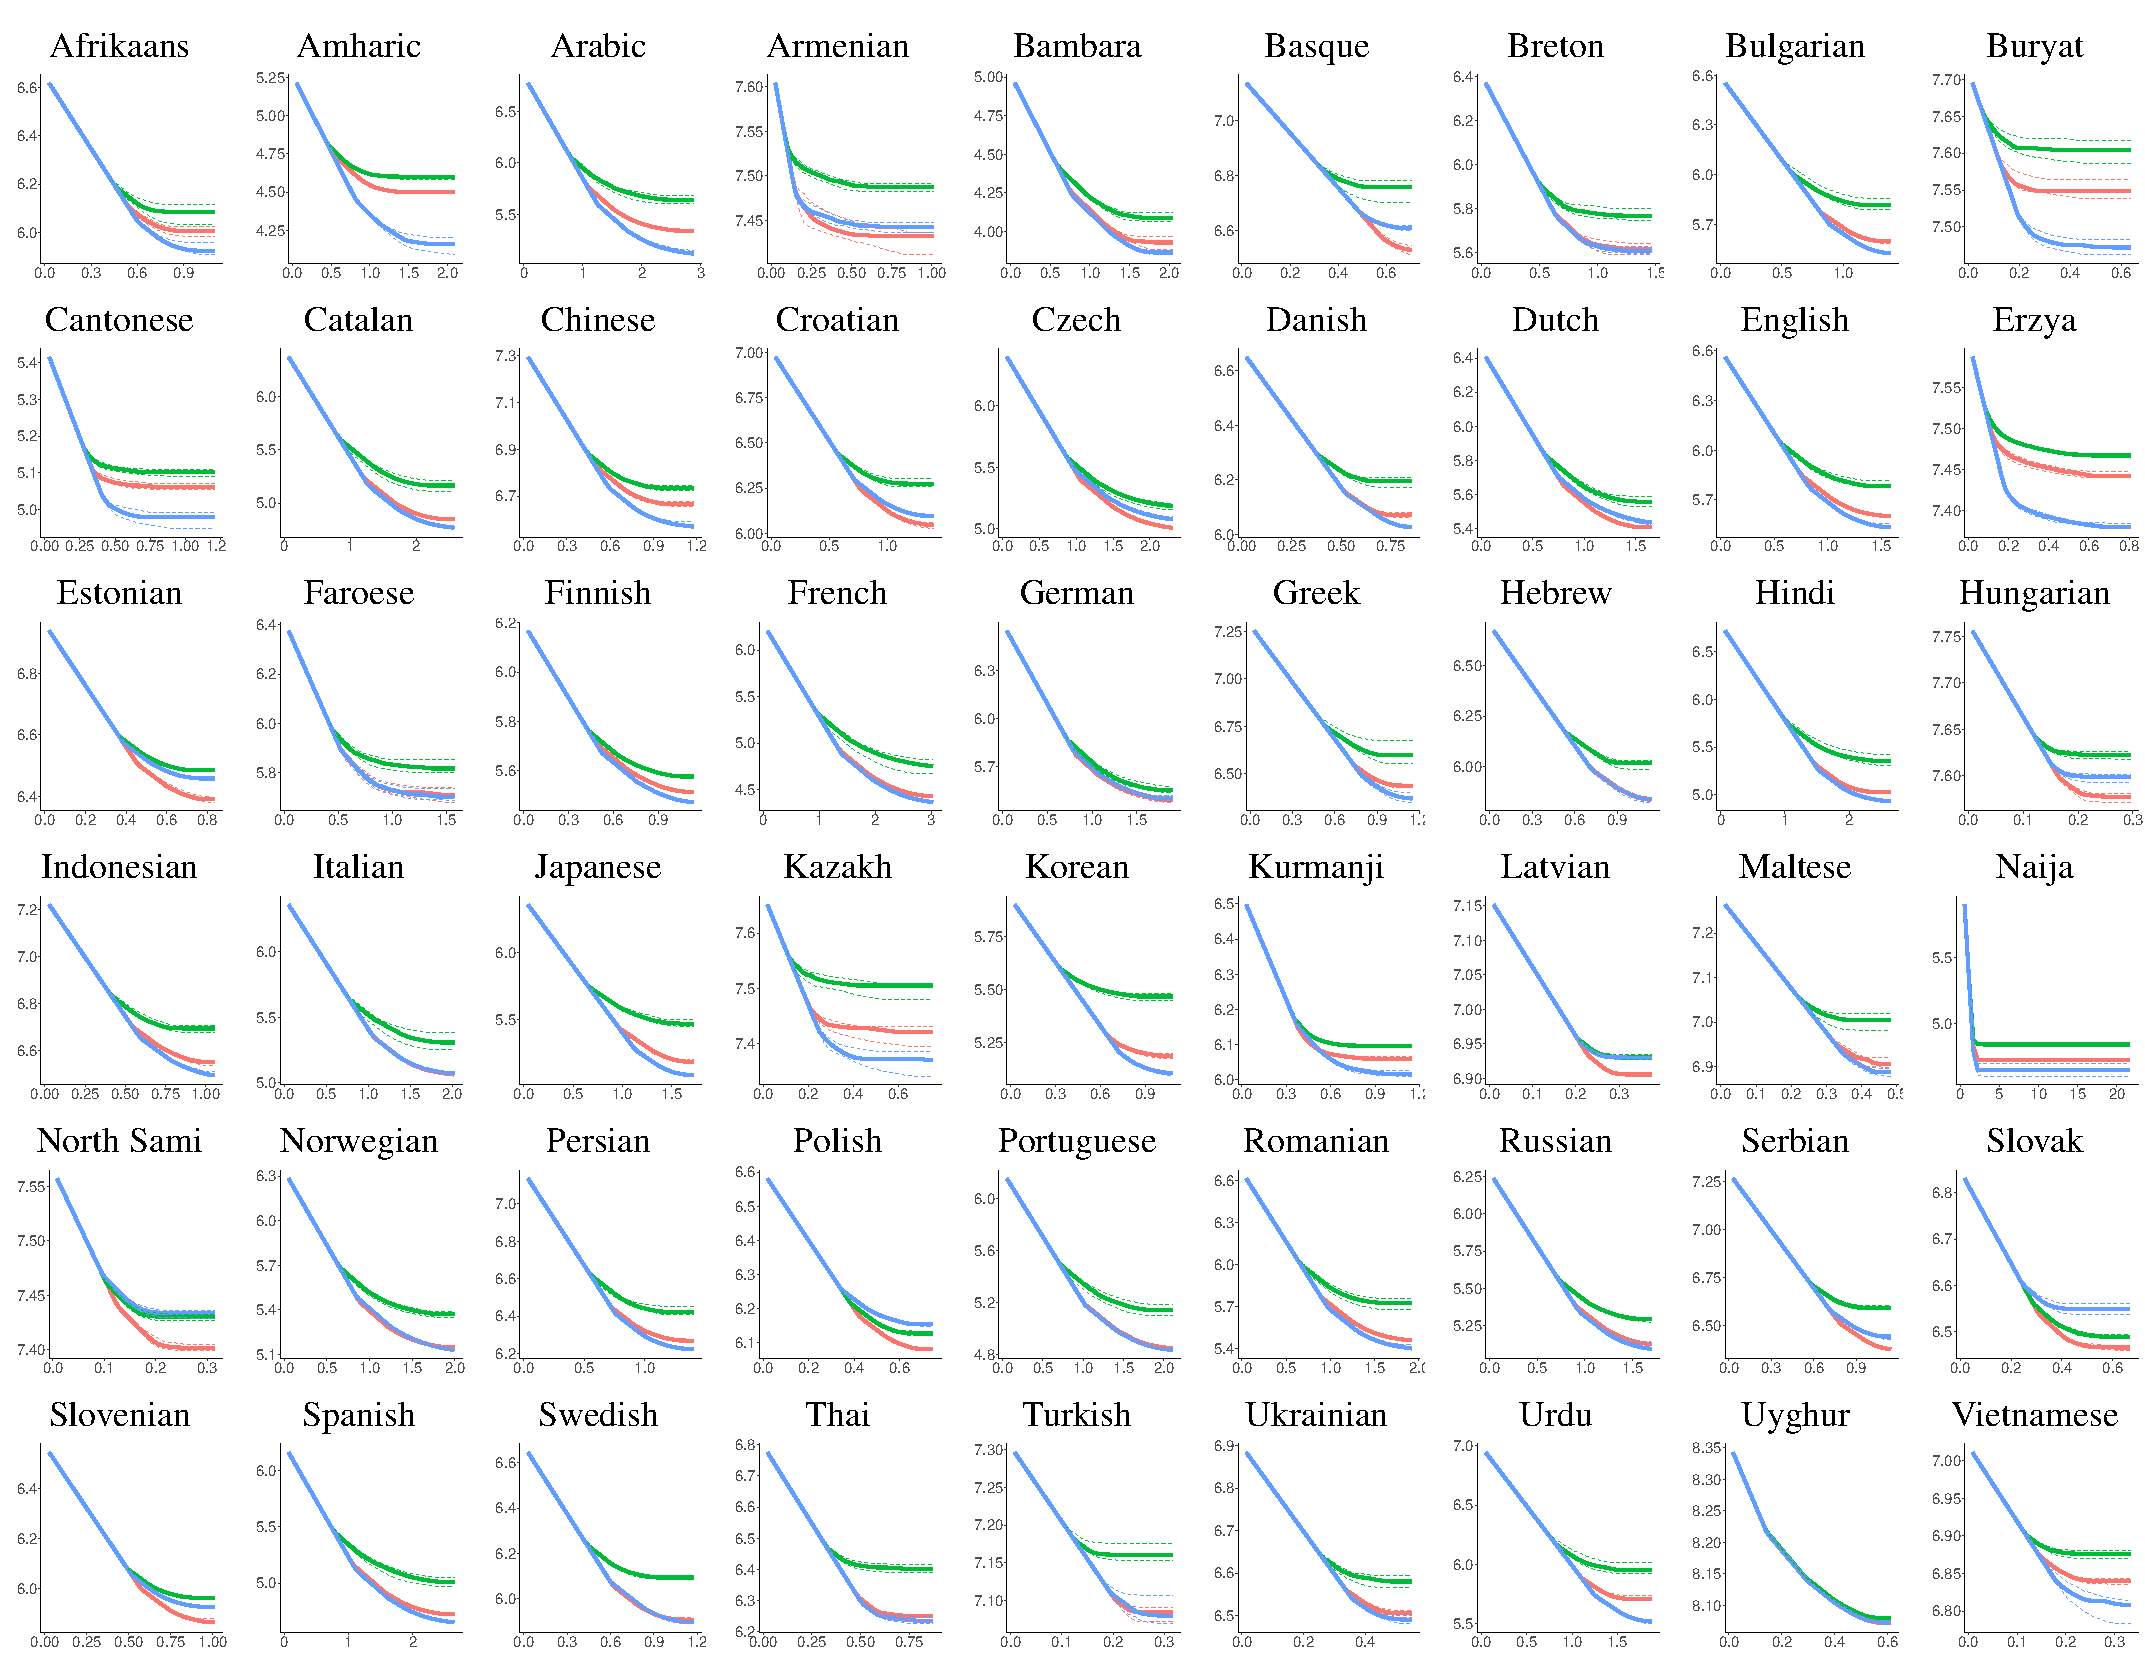
\includegraphics[width=\textwidth]{results-table-mle.pdf}
\end{center}
	\caption{Median surprisal (y-axis) at given memory level (x-axis), for real orders (blue) and random baseline grammars (red). We provide 95\% confidence bands. These are computed over different runs of the estimation algorithm for the real orders, and over different runs \emph{and} different grammars for the baseline grammars.}\label{fig:median-table}
\end{figure}



%\begin{figure}
%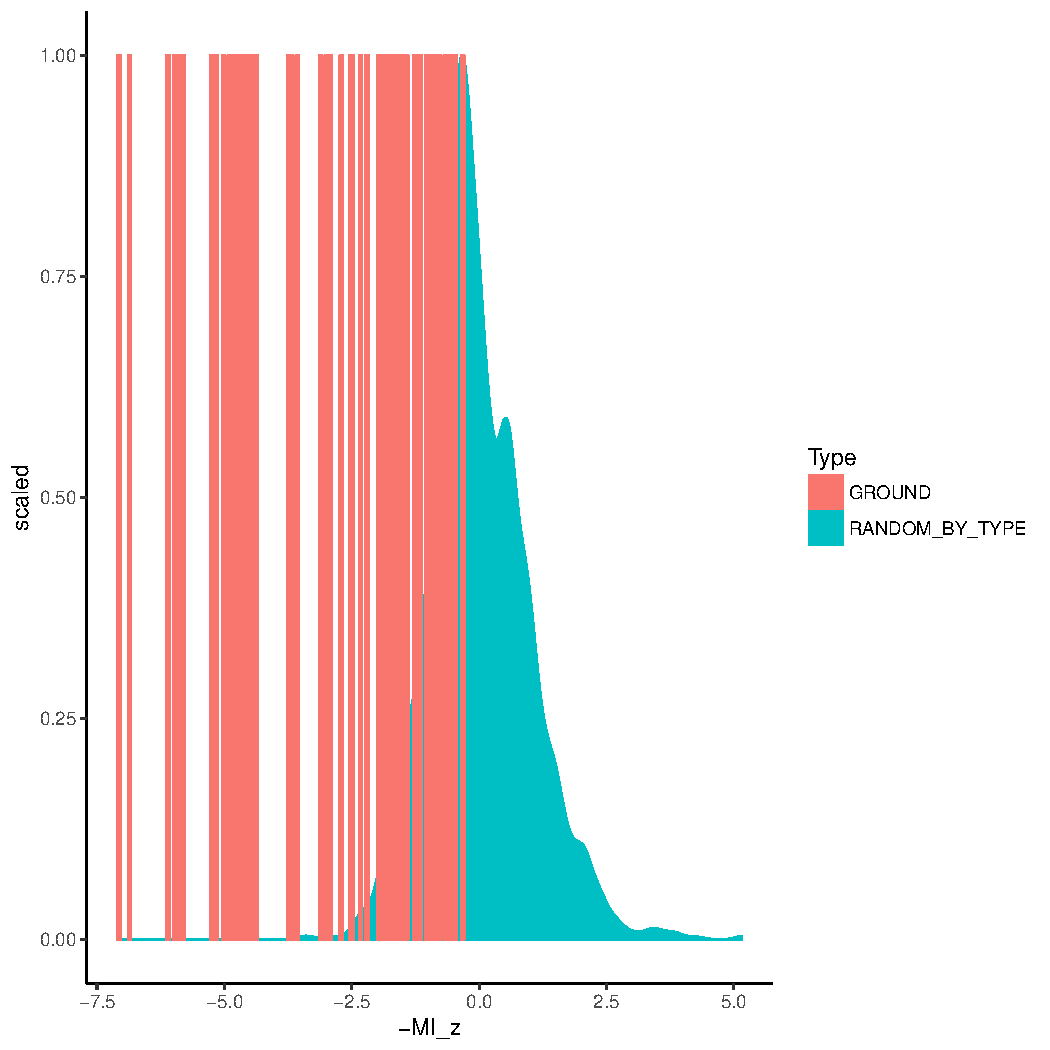
\includegraphics[width=0.5\textwidth]{figures/full-GROUND-listener-surprisal-memory-HIST_z_byMem_onlyWordForms_boundedVocab.pdf}
%	\caption{Histogram}\label{fig:hist-real}
%\end{figure}

\paragraph{Information Structure}

We show estimated tradeoffs in Figure~\ref{fig:median-czech-infostruc}.
Note that this experiment was conducted only on the subset of the Prague Dependency Treebank that has information structure annotation; thus, the numerical values are slightly different from those in Section X.




\begin{figure}
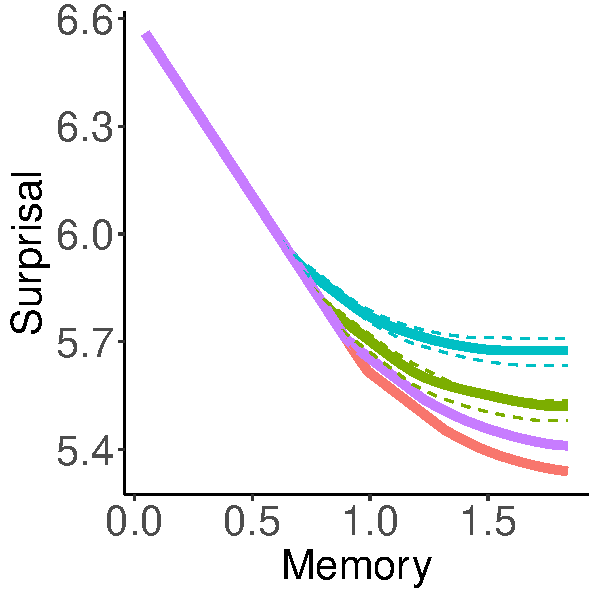
\includegraphics[width=0.5\textwidth]{figures/Czech-PDT-listener-surprisal-memory-MEDIANS_onlyWordForms_boundedVocab.pdf}
	\caption{Czech with information structure. Green: Baselines with information structure. Red: Baselines without information structure. Blue: Real}\label{fig:median-czech-infostruc}
\end{figure}



\begin{figure}
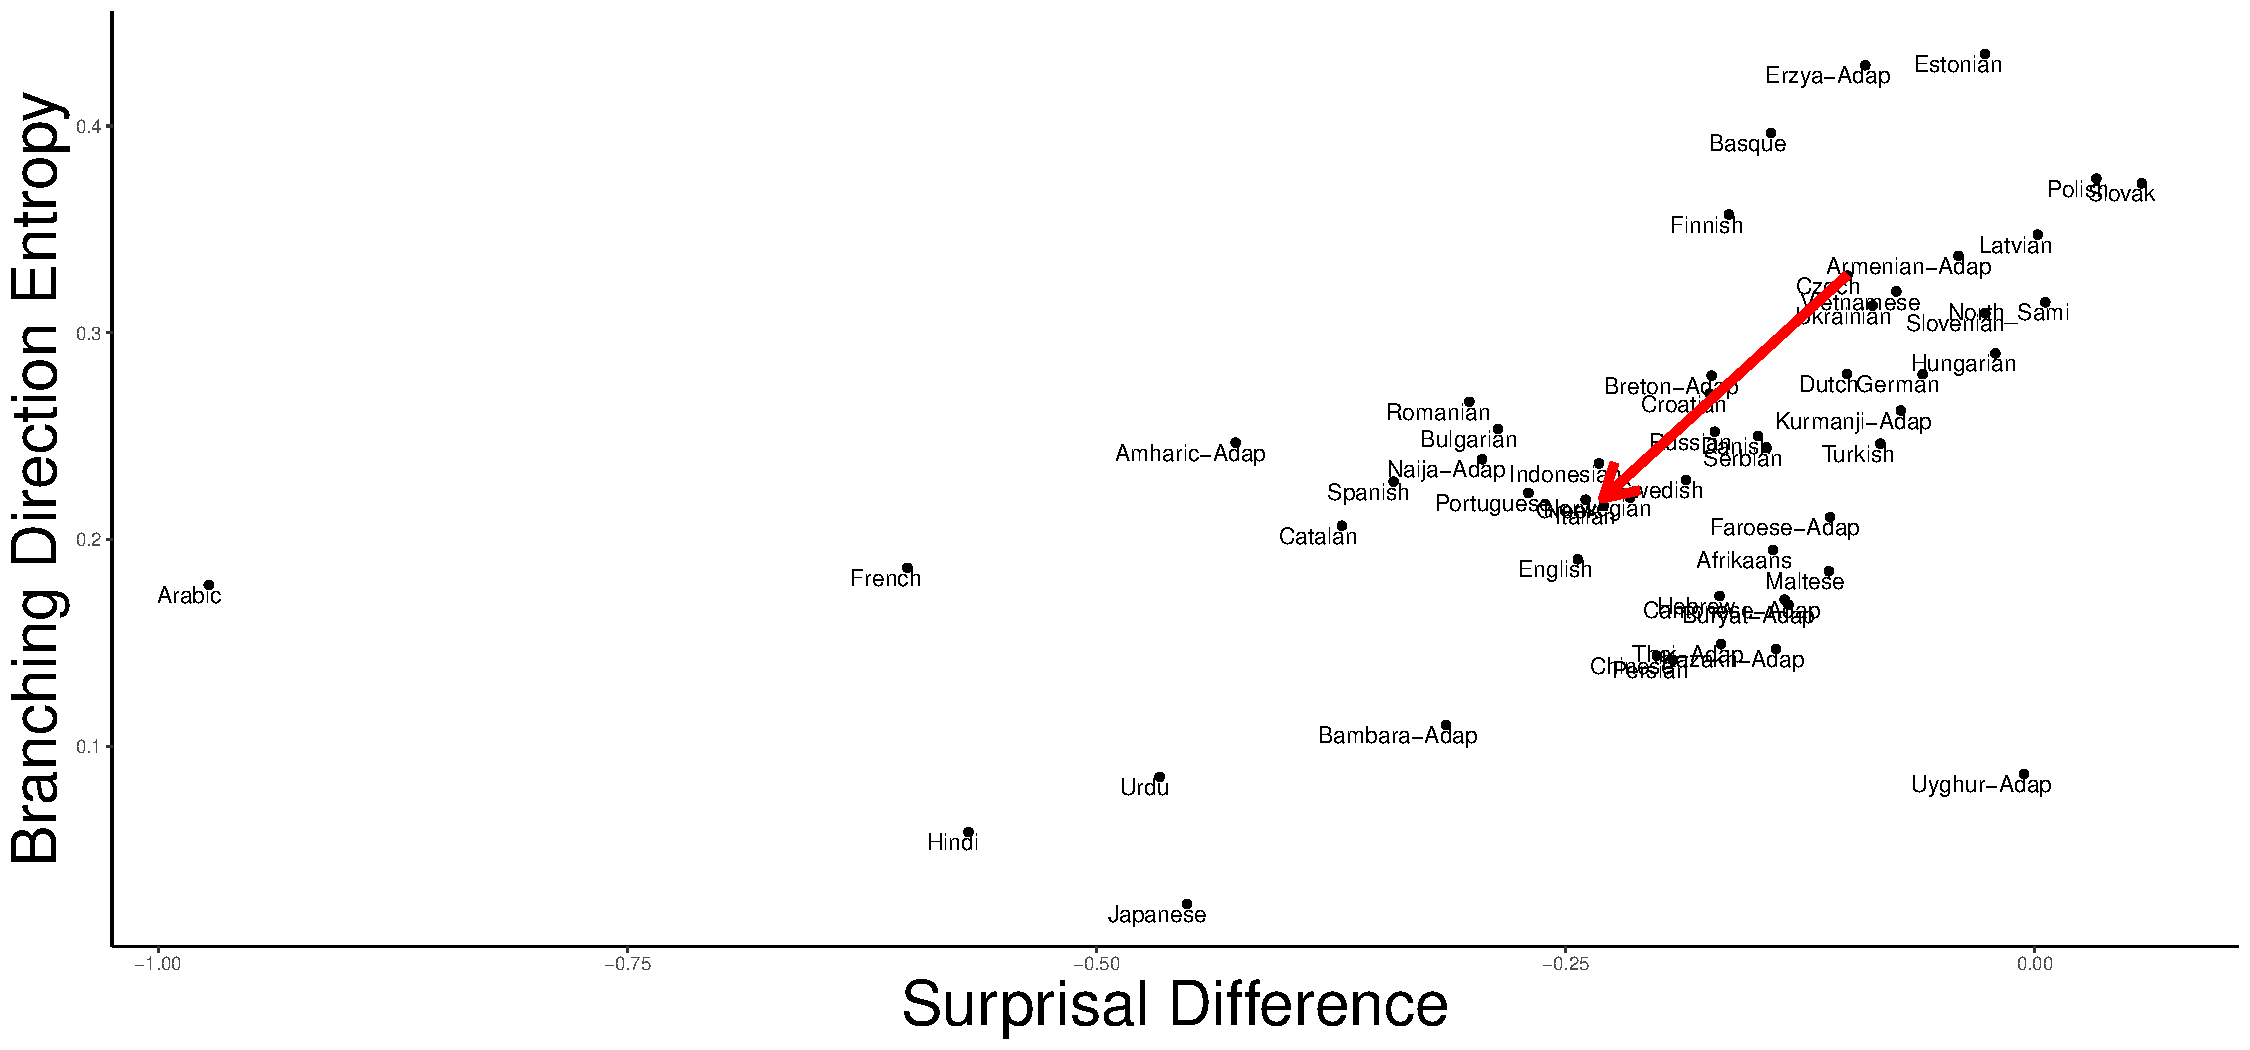
\includegraphics[width=0.9\textwidth]{figures/surprisal-branching-entropy-REAL-infostruc.pdf}
	\caption{Order Freedom vs Difference in Surprisal at maximal memory (compare Figure (REF)). The arrow indicates how the data point for Czech would move when modeling word order including information structure.
	When modeling information structure, branching direction entropy decreases, while the surprisal difference between real and baseline orders increases.
	This suggests that the weaker optimization in free word order languages observed in Experiment 2 might in part be because ordering grammars did not take information structure into account.
	}\label{fig:freedom-mi-with-infostruc}
\end{figure}




%
%\subsection{Discussion: Alternative Models}
%In view of the NLP literature, the following are the main other options that exist for estimating mutual information and probabilities in sequences:
%
%A traditional model uses n-gram models. A challenge of n-gram models is that they do not express any morphosyntactic generalizations. Furthermore, standard n-gram models do not express any generalizations about pairs of words that are not adjacent -- e.g., encoding a generalization about morphological agreement between two words is hard for such a model to capture if the two words are not always adjacent. Both the small scale of available corpora in many languages and free word order in many languages with rich morphology thus seem to make such models unattractive.
%We evaluate our hypothesis using n-gram models in SI Section X, confirming the conclusions obtained from neural models.
%
%A second option is to construct a statistical grammar, such as PCFG.
%The challenge is to encode statistical morphosyntactic generalizations, and to decide which independence assumptions to put into the model.
%One can either decide on a language-specific basis which generalizations to put in (laborious and might introduce bias), or choose a general model family that is rich enough to learn generalizations.
%The second option will make this a machine learning model that, for our purposes, does not seem to be superior to a recurrent neural network.
%



%\subsection{Data}
%\subsection{Setup}
%The recurrent neural network architecture has a range of adjustable parameters such as the number of neurons.
%For each language, we used Bayesian optimization using the Expected Improvement acquisition function (CITE) \citep{snoek-practical-2012} to find a good setting of the hyperparameters, taking average surprisal on random grammars as the objective.
%This biases the hyperparameters towards favoring counterfactual grammars.

%\subsection{Setup}




%\paragraph{Data}
%Given a sequence of input words $w_1, ..., w_n \in V$, the model 
%%
%\textbf{TODO I'm describing this in a lot of detail. Alternatively, we can say this is a standard NLP method and refer to the NLP literature for the definition.}
%The first component of such a model is an \emph{embedding matrix} $W_{emb} \in \mathbb{R}^{|V| \times d_{emb}}$, where the \emph{vocabulary} $\mathcal{V}$ is a set, containing the words that occur in the corpus, and $d_{emb} \in \mathbb{N}$ is a fixed parameter.
%This matrix assigns a $d_{emb}$-dimensional vector to each word occurring in the corpus.
%The second component is an LSTM cell $f_{LSTM}$, a nonlinear transformation mapping an \emph{input} vector $x_{i} \in \mathbb{R}^{d_{emb}}$ a \emph{hidden state} $h_i \in \mathbb{R}^{d_{LSTM}}$ and a \emph{cell state} $c_i \in \mathbb{R}^{d_{LSTM}}$ to a new pair of hidden state and cell states $h_{i+1}, c_{i+1} \in \mathbb{R}^{d_{LSTM}}$.
%The LSTM cell $f_{LSTM}$ is parameterized by a matrix of numerical parameters $W_{LSTM}$.
%
%%Such networks estimate the probability of a word in context as follows.
%Given a sequence of input words $w_1, ..., w_n \in V$, the model first retrieves fixed-dimensionality vector representations $x_1, ..., x_n$, where $x_i$ is the row of $W_{emb}$ corresponding to the word $w_i$.
%It then computes a sequence of hidden and cell states by the following recurrent computation:
%\begin{align*}
%	h_1, c_1 &:= 0 \\
%	h_2, c_2 &:= f_{LSTM}(x_1, h_1, c_1) \\
%	\dots \\
%	h_{n+1}, c_{n+1} &:= f_{LSTM}(x_n, h_n, c_n) \\
%\end{align*}
%The vector $h_i$ encodes the result of reading the words $w_1, ..., w_{i-1}$.
%We will write $LSTM(w_1, ..., w_{i-1})$ for $h_i$.
%
%The third component of the recurrent language model is the matrix $W_{output} \in \mathbb{R}^{|V| \times d_{LSTM}}$.
%We obtain per-word predictions of the next word by computing
%\begin{align*}
%	s_i := W_{output} h_i \in \mathbb{R}^{|V|} \\
%	p_i := \operatorname{softmax}(s_i)\in \mathbb{R}^{|V|} 
%\end{align*}
%where the softmax transformation normalizes vectors into probability distributions as follows
%\begin{equation}
%	\operatorname{softmax}(x)_i := \frac{\exp(x_i)}{\sum_{j=1}^{|V|} \exp(x_j)}
%\end{equation}
%Finally, the probability of the word $w_n$ in the context $w_1, ..., w_{n-1}$ is computed as
%\begin{equation}
%	p_\theta(w_n|w_1...w_{n-1}) := \frac{\exp((p_n)_{w_n})}{\sum_{w \in V} \exp(x_w)}
%\end{equation}
%and thus the surprisal is estimated as
%\begin{equation}
%- \log	p_\theta(w_n|w_1...w_{n-1}) := -\log \frac{\exp((p_n)_{w_n})}{\sum_{w \in V} \exp(x_w)}
%\end{equation}
%We discuss the choice of the numerical parameters in the next section.
%



%We collected data from the actual and random orderings in proportion one to two.
%The stopping criterion will be described below.

%Due to the randomness both in the sequence of training examples and the random initialization of the network weights, the results of the parameter estimation procedure will vary when run multiple times, especially on smaller datasets.
%Informally, due to the finiteness of the dataset, multiple parameter settings are compatible with the available training data.
%Consequently, memory-surprisal tradeoffs estimated on held-out sets will also show some variation.
%Therefore, we collect multiple samples for the actual orderings to control for variation due to the random initialization of the neural network.


%We chose these thresholds based on preliminary simulations which had suggested that these widths were achievable at acceptable computational cost.

%- at least 30 samples from both baseline and real
%
%- for the language-level tradeoff curve, either the fraction is zero or the bootstrapped CI has width $\leq 0.2$.



%
%(1) is bigram MI always greater in real languages?
%
%(2) is the tradeoff curve always lower than for deterministic simple grammar? for deterministic complex grammars? for stochastic simple/complex grammars?




%Training progresses in a series of parameter update steps, constructing updated parameters $\theta_0, \theta_1, \theta_2, \dots$.
%In the $n$-th update step, we first randomly select a word sequence $w_1 ... w_T$ from the training corpus, and use the LSTM using the current parameter setting $\theta_n$ to compute the per-word surprisals.
%We then update the parameter vector:
%\mhahn{maybe better to just say we use SGD}
%\begin{equation}\label{eq:train}
%	\theta_{n+1} := \theta_n + \alpha \partial_\theta \left(\sum_{i=1}^T \log p_\theta(w_i|w_1...w_{i-1})\right)
%\end{equation}
%where $\alpha \in \mathbb{R}_+$ is the \emph{learning rate}.

